
% This LaTeX was auto-generated from an M-file by MATLAB.
% To make changes, update the M-file and republish this document.

\documentclass{article}
\usepackage{graphicx}
\usepackage{color}

\sloppy
\definecolor{lightgray}{gray}{0.5}
\setlength{\parindent}{0pt}

\begin{document}

    
    \begin{verbatim}
clear;
close all;
im = rgb2gray(imread('circles.jpg'));
se = strel('disk',2);
afterOpening = imopen(im,se);
figure;
imshow(im);
im = afterOpening;

imBW = im2bw(im, 0.15);
figure;
imshow(imBW);

%connected components of each image
cc = bwconncomp(imBW, 8);

%label matrix of each connected component
L = labelmatrix(cc);

%num of pixels in each connected component
areasInPixels = cellfun(@length, cc.PixelIdxList);

%convert area into radius
aPix = round(sqrt(areasInPixels/pi));

%unique radii
catSize = unique(aPix);

%number of unique radii
catNum = size(catSize,2);

%number of ccs for various radii
countSz = zeros(max(catSize),1);
[sortedArea, indices] = sort(aPix);
for i = 1:length(sortedArea)
    countSz(sortedArea(i)) =  countSz(sortedArea(i)) + 1;
end
countSz = countSz(catSize);

%display circle categories based on size
disp('different cicle radii');
disp(catSize');

%display number of members in each category
for i = 1:length(catSize)
    disp([num2str(countSz(i)) ' ccs has area ' num2str(catSize(i)) ]);
end

%display which cc belongs to which category
for i = 1:size(aPix)
    disp(['cc ' num2str(i) ' belongs to ' num2str(aPix(indices))]);
end

%find ccs for each area
for i = 1:catNum
    idx = find(aPix == catSize(i));
    bw2 = ismember(L, idx);
    figure;
    imshow(bw2);
end
\end{verbatim}

        \color{lightgray} \begin{verbatim}different cicle radii
     2
     3
     4
     5
     6
     7
     8
     9
    10
    11

1 ccs has area 2
30 ccs has area 3
52 ccs has area 4
41 ccs has area 5
30 ccs has area 6
34 ccs has area 7
40 ccs has area 8
21 ccs has area 9
48 ccs has area 10
21 ccs has area 11
cc 1 belongs to 2   3   3   3   3   3   3   3   3   3   3   3   3   3   3   3   3   3   3   3   3   3   3   3   3   3   3   3   3   3   3   4   4   4   4   4   4   4   4   4   4   4   4   4   4   4   4   4   4   4   4   4   4   4   4   4   4   4   4   4   4   4   4   4   4   4   4   4   4   4   4   4   4   4   4   4   4   4   4   4   4   4   4   5   5   5   5   5   5   5   5   5   5   5   5   5   5   5   5   5   5   5   5   5   5   5   5   5   5   5   5   5   5   5   5   5   5   5   5   5   5   5   5   5   6   6   6   6   6   6   6   6   6   6   6   6   6   6   6   6   6   6   6   6   6   6   6   6   6   6   6   6   6   6   7   7   7   7   7   7   7   7   7   7   7   7   7   7   7   7   7   7   7   7   7   7   7   7   7   7   7   7   7   7   7   7   7   7   8   8   8   8   8   8   8   8   8   8   8   8   8   8   8   8   8   8   8   8   8   8   8   8   8   8   8   8   8   8   8   8   8   8   8   8   8   8   8   8   9   9   9   9   9   9   9   9   9   9   9   9   9   9   9   9   9   9   9   9   9  10  10  10  10  10  10  10  10  10  10  10  10  10  10  10  10  10  10  10  10  10  10  10  10  10  10  10  10  10  10  10  10  10  10  10  10  10  10  10  10  10  10  10  10  10  10  10  10  11  11  11  11  11  11  11  11  11  11  11  11  11  11  11  11  11  11  11  11  11
\end{verbatim} \color{black}
    
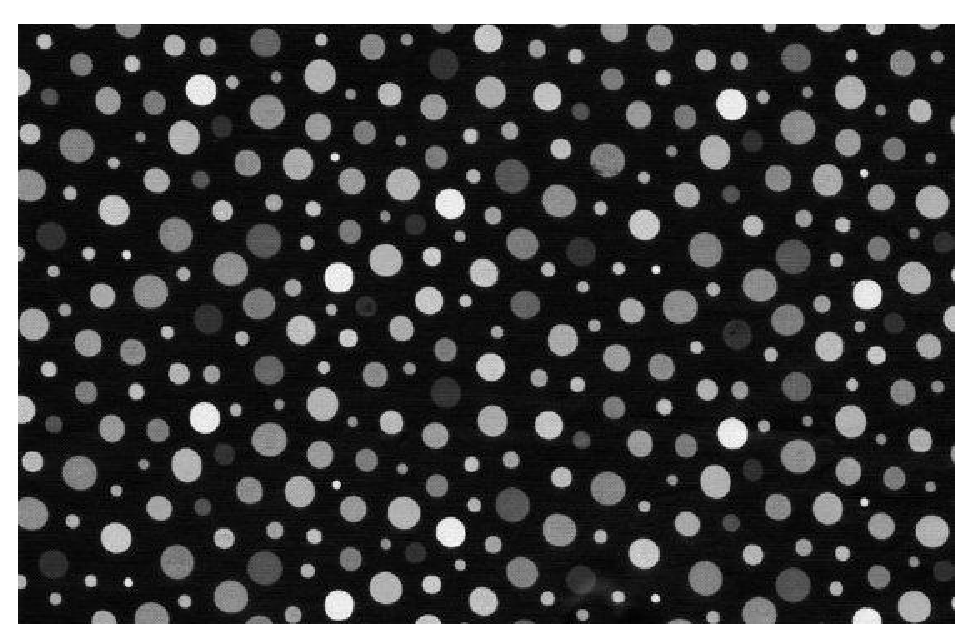
\includegraphics [width=4in]{circles2_01.eps}


\includegraphics [width=4in]{circles2_02.eps}

\includegraphics [width=4in]{circles2_03.eps}


\includegraphics [width=4in]{circles2_04.eps}


\includegraphics [width=4in]{circles2_05.eps}


\includegraphics [width=4in]{circles2_06.eps}

\includegraphics [width=4in]{circles2_07.eps}


\includegraphics [width=4in]{circles2_08.eps}


\includegraphics [width=4in]{circles2_09.eps}

\includegraphics [width=4in]{circles2_10.eps}


\includegraphics [width=4in]{circles2_11.eps}

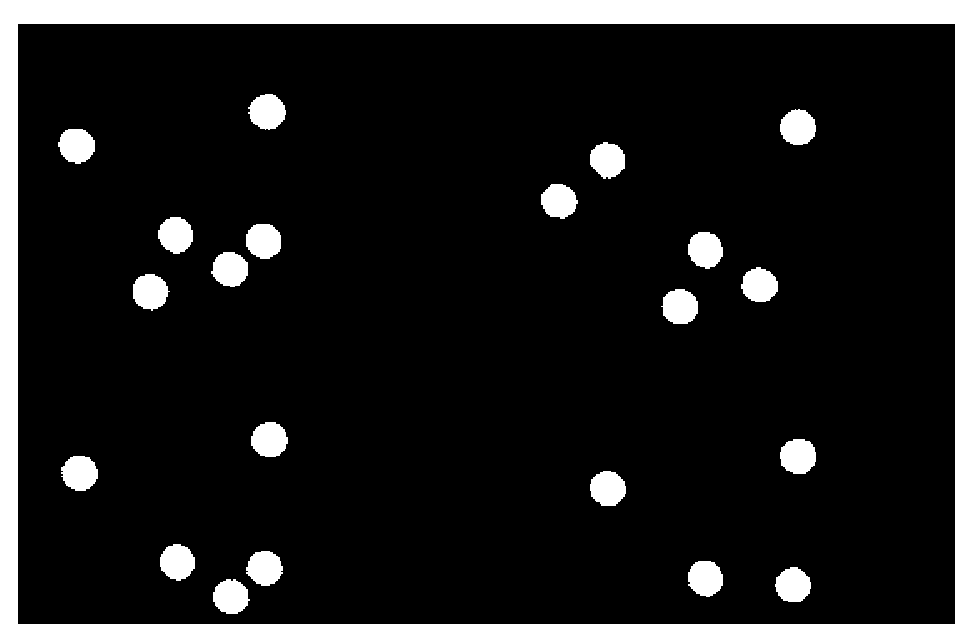
\includegraphics [width=4in]{circles2_12.eps}



\end{document}
    
